\chapter{Introduction}
\label{ch:intro}

The opening chapter of a thesis or dissertation will typically provide an introduction to the body of research. At the beginning of a chapter, it is common to provide some introductory text. Instead of discussing research, this template document will highlight how the {\ttfamily byuthesis} class and \LaTeX{} can be used to prepare a thesis or dissertation document for submission in the College of Engineering at BYU. A concise statement of the College of Engineering formatting requirements can be found in Appendix~\ref{ap:format}.

\section{Class Options}
\label{sec:class_options}
The {\ttfamily byuthesis} class has two class options. The first option allows the author to choose between a {\em simple} or {\em fancy} document format. The simple format is traditional in style and straightforward to implement using a standard word processor or \LaTeX. The fancy format leverages the advanced typesetting features of \LaTeX{} and the {\ttfamily memoir} class and more effectively utilizes the full letter-size page while following typesetting best practices. With the second class option, the author can specify whether the document fulfills the requirements for a masters or doctoral degree. For example, to use the {\ttfamily byuthesis} class for a doctoral dissertation in the simple format, the class definition (implemented on the first line of the {\ttfamily template.tex} file) would be \verb|\documentclass[simple,phd]{byuthesis}|. To create a masters thesis in the fancy format, the definition would be \verb|\documentclass[fancy,masters]{byuthesis}|. The example template document ({\ttfamily template.tex}) can be compiled using any combination of these options. Note that the simple and fancy formats use different source files for the chapters in this document. Be sure to uncomment the appropriate {\ttfamily chap*.tex} files in {\ttfamily template.tex}.

\section{Document Formatting}
\label{sec:intro_styles}
The formatting and \LaTeX{} features that you will use to prepare your thesis are outlined briefly in the next several chapters\scite{bugref1,bugref2}. The narrow, single-column format of this document is based on long-standing principles of typography.\scite{Bringhurst19} This formatting is easy to read compared to the wide-column, double-spaced format used previously for theses and dissertations. The format of the document is defined in {\ttfamily byuthesis.cls}, a \LaTeX{} class defined specifically for theses and dissertations in the College of Engineering at BYU. To give a better sense of the format of the document, we will occasionally throw in some random Latin text to take up white space. We set it apart from the text requiring your attention with a grey font color.

\myshorttexta

When using the {\ttfamily fancy} option of {\ttfamily byuthesis.cls}, footnotes appear as sidenotes in the right margin.\footnote{This is a sidenote created with the {\ttfamily $\backslash$footnote} command.} You can make a reference to a section by using its label, such as~\cref{sec:intro_styles}. You can reference a chapter in this way, for example~\cref{ch:intro}. Here is an example of a citation of a master's thesis.\scite{masters1} References for this template document are held in a file called {\ttfamily references.bib}. A complete list of the references cited in this document can be found in the References section at the end of the document before the Appendices.

\subsection{Including Figures and Tables}
The syntax above provides an example for declaring a subsection. This subsection will include some text and give an examples of figures and tables. Let's start with figures. Figures are typically diagrams, graphs, pictures, maps, or charts. Figures should be centered with respect to the text column. Figure captions should be centered below the figure.\footnote{We will introduces some alternative formats for figures and captions below that are enabled by the {\ttfamily fancy} option of the {\ttfamily byuthesis} class.} If multiple lines are needed for the caption, it should be left/right justified at the margins. Figure~\ref{fig:gradf_half_space} shows the gradient of a function and the half space where the function is decreasing. Notice how the \verb|\ref| command automatically references the correct figure number. Notice also that the \verb|~| inserts a non-breaking space, so that the label Figure and the figure number are never separated by a line break.

\begin{figure}[htbp]
	\centering
	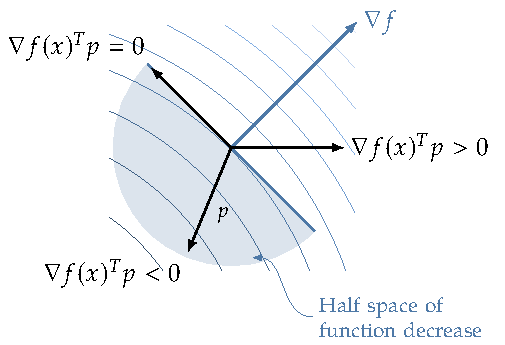
\includegraphics[width=3.0in]{gradf_half_space}
	\caption{This is a regular figure with a centered bottom caption.}
	\label{fig:gradf_half_space}
\end{figure}

\myshorttexta

\begin{marginfigure}
	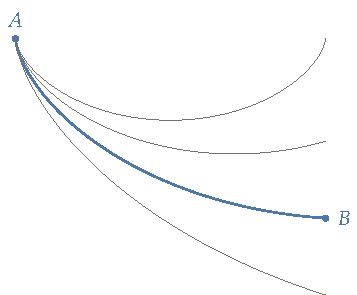
\includegraphics[width=1.8in]{brachistochrone}
	\caption{This is an example of a margin figure.}
	\label{fig:brach}
\end{marginfigure}

Figures should be placed after the paragraph in which they are first referenced. If a figure will not fit on the same page, continue the text and place the figure at the top of the next page. With the {\ttfamily byuthesis.cls} document class, we can have small figures that are set in the sidemargin. Figure~\ref{fig:brach} is an example of a margin figure.

\myshorttext

We can also create figures that place the caption in the side margin. Figure~\ref{fig:sidecap} is an example of this. This is a matter of personal preference. You can choose between centered captions and side-margin captions, but you should be consistent throughout your document.
\begin{figure}[htbp]
	\begin{sidecaption}{This is a figure with a side caption that is not short, but not that long either.}[fig:sidecap]
		\centering
		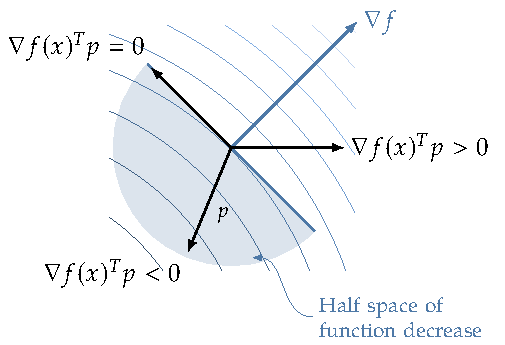
\includegraphics[width=3.0in]{gradf_half_space}
	\end{sidecaption}
\end{figure}

Finally, we can create a figure that spans the width of the text column and the side margin\scite{bugref1} as shown in Figure~\ref{fig:fullwidth}. This option should not be used frequently as it requires some tweaking of the vertical distance of the caption and follow-on text below the figure. It will work robustly when the figure appears at the top or middle of a page, but may push the caption onto the next page when it appears at the bottom. There may be some instances with wide images where the additional manual adjusting is worth the effort.

\begin{figure}[h]
	\setlength{\sidecapraise}{-1.3cm}   % manual adjustment of figure caption position
	\begin{sidecaption}{The caption for a full-width figure appears in the margin below it.}[fig:fullwidth] %Such figures utilize the side margin.}
		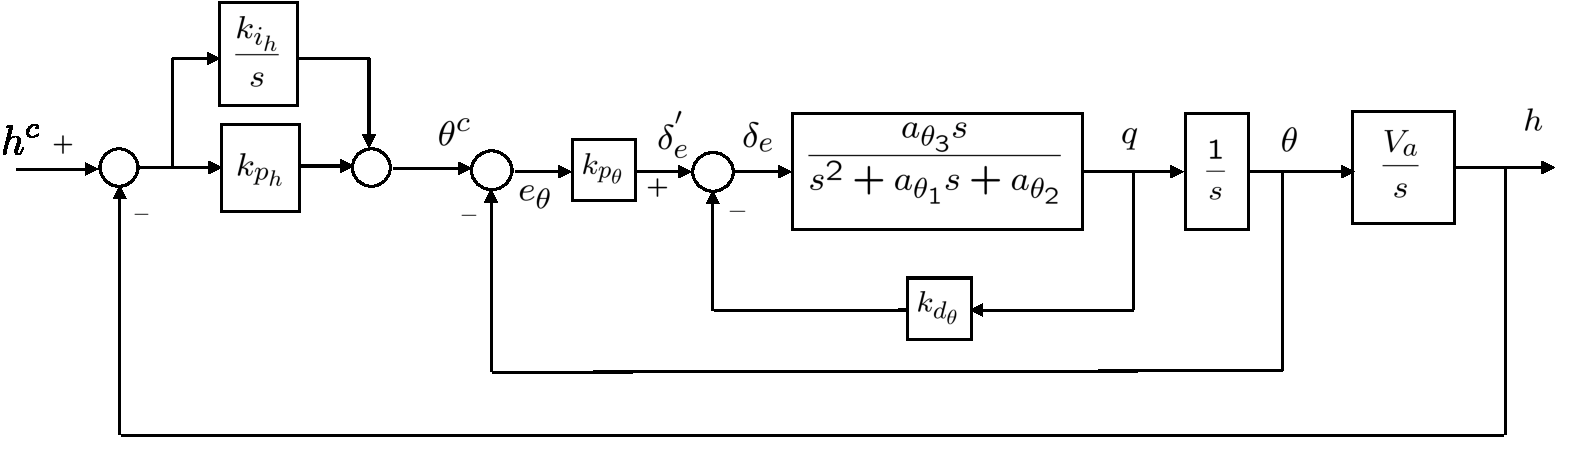
\includegraphics[width=6.5in, inner]{altitude-pitch-all}
	\end{sidecaption}
	\vskip -1.0cm     % manual adjustment of position of main text below figure. Only needed because of the extra space introduced by the subsubsection command that immediately follows this figure.
\end{figure}

\subsubsection{Subsubsection Example}
The syntax above provides an example of how to include a subsubsection. In this thesis template, the document has four primary division levels: \verb|\chapter|, \verb|\section|, \verb|\subsection|, and \verb|\subsubsection|. The command \verb|\subsubsection| is used to define the lowest level of division. Notice that subsubsection titles are not numbered.

\subsubsection{Including Tables}
Tables typically contain numerical or statistical information. Tables are also fairly straightforward to include in a \LaTeX{} document. Table~\ref{tab:table_example} shows a simple table. Tables are most commonly centered in the text column with the table caption centered above the table. If more than one line is needed for the caption it should be justified at the text margins as shown in Table~\ref{tab:table_example}.

\LaTeX{} refers to figures and tables as floats and often tries to locate figures at the top or bottom of a page. The user has some control over this, but \LaTeX{} can behave like it has a mind of its own sometimes. In reality it is placing figures according to internal algorithms and parameters that you can adjust. If you are interested in digging into this level of detail, an internet search on ``LaTeX float parameters'' will provide ample reading.  In creating the table, we have used the command \verb|\begin{table}[t]|. The parameter \verb|[t]| allow us to specify preference for the location of table to be at the \emph{top} of the page.

\begin{table}[t]
	\centering
	\caption[This is a standard table with a top caption.]{This is a standard table with a top caption. More text is included in the title to show how multi-line titles should be left and right justified with the text column margins.}
	\label{tab:table_example}	\begin{tabular}{ c c c c}
		\toprule
		basin & curve \\
		name & number & minimum & maximum \\
		\midrule
		1B & 68.5 & 49.2 & 84.1 \\
		2B & 66.2 & 46.8 & 82.7 \\
		3B & 65.4 & 45.5 & 82.3 \\
		\midrule
		average & 66.7 & 47.2 & 83.0 \\
		\bottomrule
	\end{tabular}
\end{table}

Table~\ref{tab:table_sidecaption} shows an example of the same table using a side caption. We have used the placement preferences \verb|[bht]| to give first preference to the \emph{bottom} of the page, second preference to the current positioning in the source code (\emph{here}), and third preference to the \emph{top} of the page. As you can see, \LaTeX{} may override our preferences, based on the space available and its typesetting rules.

\begin{table}[bht]
	\begin{sidecaption}{This is a standard table with a side caption.}[tab:table_sidecaption]
		\centering
		\begin{tabular}{ c c c c}
			\toprule
			basin & curve \\
			name & number & minimum & maximum \\
			\midrule
			1B & 68.5 & 49.2 & 84.1 \\
			2B & 66.2 & 46.8 & 82.7 \\
			3B & 65.4 & 45.5 & 82.3 \\
			\midrule
			average & 66.7 & 47.2 & 83.0 \\
			\bottomrule
		\end{tabular}
	\end{sidecaption}
\end{table}

Notice that in the tables above, we have eliminated the vertical rules separating the columns. Doing so creates tables that are less cluttered and easier to read. If a table is to occupy a full page in landscape format, the top of the table should be on the left side of the page, with the caption above the table.

\subsection{Formatting Equations}
Equation formatting is one of \LaTeX's most useful features\scite{bugref1} and a good reason why it is often used for theses and dissertations in the College of Engineering. It is easy to format equations within a sentence, such $c = 2 \pi r$ to describe the circumference of a circle. Equations should be treated as part of the text. As an example, the surface area of a cylinder is given by
\begin{equation}
	\label{eq:surface_area_cyl}
	S = 2\pi r \left( r + h \right) ,
\end{equation}
where $r$ is the radius of the cylinder and $h$ is its height. The area of a circle can be expressed in terms of its diameter $d$ as
\begin{equation}
	\label{eq:area_circle}
	A = \frac{\pi}{4} d^2 .
\end{equation}

Often, it is desirable to align a sequence of equations. Again, \LaTeX{} makes this pretty easy. The roots of the polynomial function $f(x)$ can be found by factoring
\begin{align}
	f(x) &= x^3 + 5x^2 + 6x \\
		 & = x (x^2 + 5x + 6) \\
		 & = x (x + 2)(x +3) ,
\end{align}
setting each of the factors to zero, and solving for $x$. Equations without numbers can be typeset like this
\[
	x = a + b
\]
or like this
\begin{equation*}
	y = c + d .
\end{equation*}
Just as we did with sections, figures, and tables, we can reference a specific equation by using its declared label. In~\eqref{eq:surface_area_cyl}, the surface area of a cylinder is defined. Another format would be to say Equation~\ref{eq:area_circle} defines the area of a circle. Yet another format is \cref{eq:area_circle}. Any of these formats is acceptable. Use just one of them and be consistent.

\LaTeX{} can do so much with the typesetting of equations. These few examples are just a small sampling of its impressive capabilities.

\myshorttexta 

\section{Invoking the bug}

Invoking the bug requires a number of pages\scite{bugref1}. This makes sense, since it only manifests when there are too many pages in the cited by lists.
